\documentclass[sigconf,anonymous,review]{acmart}

% IMPORTANT: the official AAMAS 2027 template download returned HTTP 404 on
% 2026-09-13. Replace this class/metadata with the repaired official package
% before submission; do not modify its layout parameters.

\usepackage{booktabs}
\usepackage{amsmath,amssymb,mathtools}
\usepackage{algorithm}
\usepackage{algpseudocode}
\usepackage{tikz}
\usetikzlibrary{arrows.meta,positioning,fit,backgrounds,calc}
\usepackage{pgfplots}
\pgfplotsset{compat=1.18}

\newtheorem{proposition}{Proposition}
\newtheorem{lemma}{Lemma}
\newcommand{\calms}{\textsc{Calm-S}}
\newcommand{\ind}{\mathbb{I}}
\DeclareMathOperator*{\argmaxop}{arg\,max}

\setcopyright{none}
\acmConference[AAMAS 2027]{The 26th International Conference on Autonomous Agents and Multiagent Systems}{May 3--7, 2027}{Hanoi, Vietnam}
\acmYear{2027}
\copyrightyear{2027}
\acmISBN{}
\acmDOI{}

\begin{document}

\title{CALM-S: Audited Forecast Settlement for Budgeted LLM-Agent Orchestration}

\author{Anonymous Author(s)}
\affiliation{\institution{Anonymous Institution}}

\begin{abstract}
Markets for large-language-model (LLM) agents increasingly allocate work using
reported confidence, price, or reputation. A report that influences selection,
however, is usually evaluated only after the reporting agent is selected. This
endogeneity creates two problems: a proper scoring rule need not make the report
truthful once it also changes allocation, and outcomes for unselected
task--worker pairs are selectively missing. We introduce \calms{}, a separation
layer for budgeted workflow orchestration. Workers report cost and availability;
independent forecasters report outcome distributions; a report-independent audit
stream gives every pair positive observation probability; and forecasters are
settled by inverse-propensity proper scores. Delayed audit-only weights feed a
receding-horizon optimizer over a task DAG. We prove truthfulness of the audit
score under explicit no-side-interest assumptions, unbiasedness of the settled
score, and a decision-regret sensitivity bound. In a reproducible controlled
simulation (30 seeds, 80 episodes each), an adaptive independent pool achieves
14.427$\pm$0.204 net value versus 12.851$\pm$0.141 for a static router under a
declared shift, while a coupled self-report policy achieves 12.045$\pm$0.220.
Yet two audits per episode reduce net value to 14.182$\pm$0.201: auditing is
incentive-relevant but not free. A separate strategic experiment shows that
inflation is profitable when reports control selection (0.741 vs. 0.476 payoff)
but not under separated audit settlement (0.761 vs. 0.791). These are simulator
pre-results, not claims about deployed LLMs; we specify the preregistered
real-model study required to test external validity.
\end{abstract}

\keywords{LLM agents, multiagent systems, mechanism design, proper scoring rules, task allocation, selective labels, orchestration}

\maketitle

\section{Introduction}

LLM systems can choose among workers that differ sharply by task, latency, and
price. Recent work already treats this as an economic allocation problem. Agora
decomposes a request into a graph, calibrates self-confidence, auctions task
units, executes them, and refines the calibrator online~\cite{zhou2026agora}.
AgentLance implements a repeated labor market with private cost bids, public
reputation, VCG-style payments, and subcontracting~\cite{liu2026agentlance}.
Agent Exchange (AEX) studies multi-attribute and combinatorial auctions with
settlement~\cite{yang2025aex}. Consequently, neither ``auctioning LLM work'' nor
``closing the orchestration loop'' is a defensible novelty claim.

We study a narrower failure hidden inside these loops. Suppose a worker reports
success probability $q$. A high $q$ makes selection more likely, and only the
winner's outcome is observed. Paying a proper score after execution is not enough:
the report changes whether the scoring event occurs. Moreover, updating a
calibrator on winners alone creates a selective-label problem~\cite{lakkaraju2017selective}.
The mechanism can favor a confident worker, observe only that worker, and then use
the resulting evidence to validate its original preference.

\calms{} separates the labor and information roles (Fig.~\ref{fig:loop}). Workers
offer cost and capacity; independent forecasters predict each task--worker
outcome. A small, report-independent audit stream executes shadow assignments
with logged propensities. Audit outcomes settle forecasters through a strictly
proper rule~\cite{gneiting2007proper}; delayed audit-only performance weights then
enter the allocator. This borrows the separation principle of two-stage forecast
elicitation~\cite{papakonstantinou2008truthful}, but addresses LLM workflow
allocation and selectively observed task--worker outcomes.

Our contributions are:
\begin{enumerate}
  \item a diagnosis and counterexample showing why winner-only proper scoring
  does not imply truthful self-confidence;
  \item \calms{}, an audit-supported separation layer for forecast settlement and
  budgeted task-DAG allocation;
  \item truthfulness, unbiased-score, and decision-sensitivity results under
  stated assumptions; and
  \item reproducible controlled pre-experiments plus a preregistered real-LLM
  protocol. The pre-experiments include a negative result: the tested audit rate
  costs more than its measured routing benefit.
\end{enumerate}

\begin{figure*}[t]
\centering
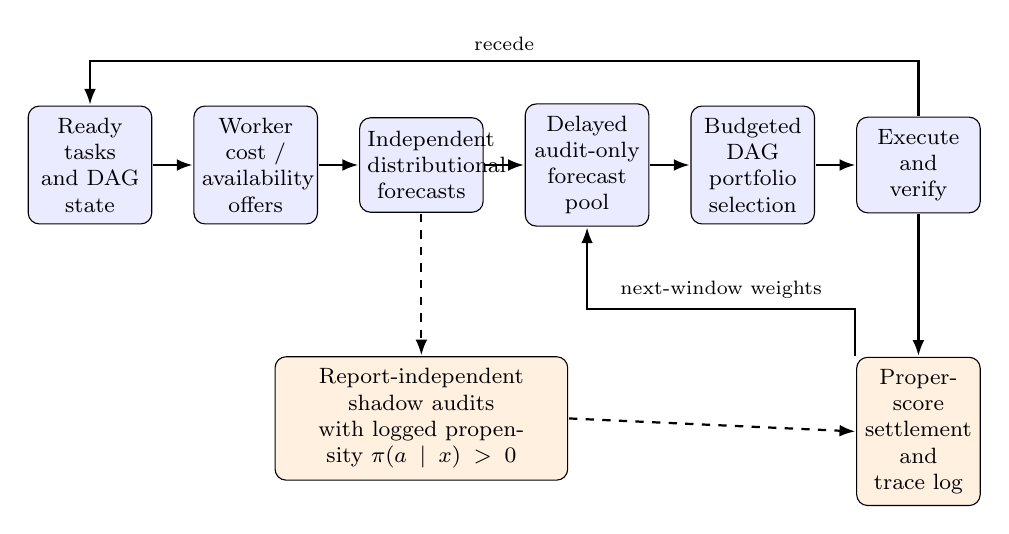
\begin{tikzpicture}[
  node distance=18mm and 5mm,
  box/.style={draw,rounded corners,align=center,minimum height=12mm,
    text width=\dimexpr(\textwidth-25mm)/6-2mm-1pt\relax,
    inner xsep=1mm,inner ysep=1.5mm,outer sep=.5pt,font=\footnotesize},
  main/.style={box,fill=blue!8}, audit/.style={box,fill=orange!12},
  arr/.style={-{Latex[length=2mm]},thick}, dashedarr/.style={arr,dashed}
]
\node[main] (tasks) {Ready tasks\\and DAG state};
\node[main,right=of tasks] (cost) {Worker cost /\\availability offers};
\node[main,right=of cost] (forecast) {Independent\\distributional forecasts};
\node[main,right=of forecast] (pool) {Delayed audit-only\\forecast pool};
\node[main,right=of pool] (select) {Budgeted DAG\\portfolio selection};
\node[main,right=of select] (execute) {Execute and\\verify};
\node[audit,text width=.29\textwidth,below=18mm of forecast] (audit) {Report-independent shadow audits\\with logged propensity $\pi(a\mid x)>0$};
\node[audit,below=18mm of execute] (settle) {Proper-score\\settlement\\and trace log};
\draw[arr] (tasks)--(cost);
\draw[arr] (cost)--(forecast);
\draw[arr] (forecast)--(pool);
\draw[arr] (pool)--(select);
\draw[arr] (select)--(execute);
\draw[dashedarr] (forecast.south)--(audit.north);
\draw[dashedarr] (audit.east)--(settle.west);
\draw[arr] (execute.south)--(settle.north);
\draw[arr] (settle.north west) -- ++(0,6mm)
  -| node[pos=.25,above,font=\scriptsize]{next-window weights} (pool.south);
\draw[arr] (execute.north) -- ++(0,7mm)
  -| node[pos=.25,above,font=\scriptsize]{recede} (tasks.north);
\end{tikzpicture}
\caption{\calms{} separates work allocation (top) from report-independent audit
settlement (bottom). Solid arrows are the operating loop; dashed arrows are the
audit channel. Forecast weights change only after an audit window settles.}
\Description{A flow diagram from tasks to worker offers, independent forecasts,
forecast pooling, portfolio selection, execution, and settlement, with a
separate randomized audit path from forecasts to settlement.}
\label{fig:loop}
\end{figure*}

\section{Related Work and Novelty Boundary}

\paragraph{LLM orchestration and routing.}
Role-pipeline systems such as MetaGPT coordinate specialized LLM agents through
fixed workflows~\cite{hong2024metagpt}. Cost-aware routers such as FrugalGPT trade
quality against inference cost~\cite{chen2024frugalgpt}, while RACER adds
calibrated risk control~\cite{hao2026racer}. Agora is the closest orchestration
system: it already contains graph planning, confidence calibration, auction-based
allocation, and refinement~\cite{zhou2026agora}. \calms{} does not claim those
ingredients; it targets endogenous scoring and selective outcome collection.

\paragraph{Agent markets and credit.}
Contract Net initiated market-style distributed task allocation~\cite{smith1980contract},
and market-based multi-robot allocation has a large literature~\cite{dias2006market}.
AgentLance and AEX bring labor-market and exchange designs to LLM agents
\cite{liu2026agentlance,yang2025aex}. Shapley-Coop prices marginal contribution
after collaboration~\cite{hua2025shapley}. Our setting differs from post-hoc
credit: a separate information supplier predicts execution outcomes before
allocation and is settled on report-independent audits.

\paragraph{Forecast elicitation and selective labels.}
Strictly proper rules elicit beliefs when the event and payment exposure are
fixed~\cite{gneiting2007proper}. Principal--agent scoring mechanisms can also
incentivize costly information acquisition~\cite{chen2023principal}.
Papakonstantinou et al. separate procurement of a forecast from scoring it
\cite{papakonstantinou2008truthful}. \calms{} applies this separation to many
task--worker alternatives whose counterfactual outcomes are normally missing,
connecting mechanism design to selective-label evaluation
\cite{lakkaraju2017selective}. We claim novelty only for this combination and its
agent-orchestration study, not for scoring rules, auctions, calibration, or DAG
optimization individually.

\section{Model and Failure of Coupled Scoring}

An episode has task DAG $G=(V,E)$, workers $W$, forecasters $M$, and budget $B$.
Task $v$ has a machine-verifiable outcome $Y_{vw}\in\{0,1\}$ if executed by
worker $w$, with true probability $p_{vw}$. Public execution cost is $c_{vw}$;
a private-cost extension may use a separately valid procurement mechanism. A
completed set and outcomes produce value $u$, which may be additive, thresholded,
or bottlenecked. An allocation $a$ assigns workers to a feasible subset and has
true objective
\begin{equation}
F(a;p)=\mathbb{E}_{Y\sim p}[u(a,Y)]-\sum_{(v,w)\in a}c_{vw},
\quad \sum c_{vw}\le B.
\end{equation}

Forecaster $m$ reports $q_{mvw}$. In a \emph{coupled} design the same report
changes the probability of selecting $(v,w)$ and is scored only if selected.

\begin{lemma}[Winner-only scoring can reward inflation]\label{lem:coupled}
Let a report $q$ be selected iff $q\ge\tau$, and let selected payoff be
$b+S(q,Y)$, where $S$ is strictly proper and $b>0$. For any belief $p<\tau$,
there exist $b$ and $q'\ge\tau$ such that reporting $q'$ gives higher expected
payoff than truthful reporting $p$.
\end{lemma}
\begin{proof}
Truthful reporting is not selected and pays zero. Strict properness makes
$\Delta=\mathbb{E}_p[S(p,Y)-S(q',Y)]>0$, but choosing
$b>-\mathbb{E}_p[S(q',Y)]$ gives $\mathbb{E}_p[b+S(q',Y)]>0$. Thus the extensive-margin benefit
of selection can dominate the scoring loss.
\end{proof}

The point is not that proper scores fail; their fixed-exposure assumption fails.
The numerical counterexample in Section~\ref{sec:pre} shows the effect at scale.

\section{CALM-S}

\subsection{Separated reports and audited settlement}

Workers provide cost and availability, not current-task success probabilities.
Forecasters have no ownership of workers and no utility from the chosen
allocation beyond their declared score payment. Before allocation they report
$q_{mvw}$ for all candidates. The mechanism draws shadow audits from a policy
$\mu(a\mid x)$ fixed independently of current reports, with
$\pi_{a}=\Pr(Z_a=1\mid x)>0$. Audit execution does not change project value.

For the quadratic score $S(q,y)=1-(q-y)^2$, audit settlement is
\begin{equation}\label{eq:ips}
P_m=P_0+\beta\sum_{a}\frac{Z_a}{\pi_a}S(q_{ma},Y_a).
\end{equation}
Other strictly proper scores can replace $S$; continuous time/cost forecasts can
use proper distributional scores. Unclipped inverse propensities preserve the
result below but may have high variance, so clipping must be an explicit biased
ablation rather than an undocumented implementation detail.

\begin{proposition}[Audit truthfulness]\label{prop:truth}
Assume risk-neutral forecasters, report-independent audits with $\pi_a>0$, no
allocation-side utility, and outcomes distributed according to forecaster belief
$p_{ma}$. Expected payment in Eq.~\eqref{eq:ips} is uniquely maximized by
$q_{ma}=p_{ma}$ for every $a$.
\end{proposition}
\begin{proof}
Independence gives
$\mathbb{E}[Z_a S(q,Y_a)/\pi_a]=\mathbb{E}[S(q,Y_a)]$.
Strict properness uniquely maximizes each summand at the belief $p_{ma}$.
\end{proof}

\begin{proposition}[Unbiased audit score]\label{prop:unbiased}
For any fixed reports, the inverse-propensity audit estimator in
Eq.~\eqref{eq:ips} is unbiased for the full-information sum of expected scores.
\end{proposition}
This Horvitz--Thompson identity is simple but operationally important: selected
outcomes alone estimate performance on the allocator's endogenous action
distribution, not on all candidate pairs.

\subsection{Pooling, allocation, and delayed updates}

Let $\ell_{ma}$ be audit Brier loss settled before the current window. We use
regional exponential weights
\begin{equation}
\omega_{ma}\propto\exp(-\eta\bar\ell_{ma}),\qquad
\hat p_a=\sum_m\omega_{ma}q_{ma}.
\end{equation}
This is a design choice, not a theorem that calibration weighting always helps.
Equal weights, stacking, and Bayesian pooling are mandatory ablations. Given
$\hat p$, the allocator approximately solves $\argmax_a F(a;\hat p)$ over
precedence-, capacity-, and budget-feasible allocations. Only the first bounded
bundle executes; matured outcomes settle; the horizon then recedes.

\begin{proposition}[Decision sensitivity]\label{prop:regret}
Let $a^*=\argmax_a F(a;p)$, and let $\hat a$ be an $\epsilon_{\mathrm{opt}}$-
optimal solution under $\hat p$. If
$\sup_a|F(a;p)-F(a;\hat p)|\le\epsilon_p$, then
$F(a^*;p)-F(\hat a;p)\le2\epsilon_p+\epsilon_{\mathrm{opt}}$.
\end{proposition}
\begin{proof}
Insert $F(a^*;\hat p)$ and $F(\hat a;\hat p)$ between the two true objectives,
apply the uniform error bound twice, and use approximate optimality.
\end{proof}

\begin{algorithm}[t]
\caption{One \calms{} decision window}\label{alg:calm}
\begin{algorithmic}[1]
\State collect worker costs/capacity and independent forecasts $q_{m,a}$
\State pool with weights settled before this window
\State choose a feasible DAG bundle under remaining budget
\State log state, candidates, reports, propensities, and chosen bundle
\State execute chosen work; independently draw and execute shadow audits
\State verify outcomes and settle forecasters by Eq.~\eqref{eq:ips}
\State update weights only when the audit window matures; replan
\end{algorithmic}
\end{algorithm}

\section{Controlled Pre-Experiments}\label{sec:pre}

\subsection{Design}

We built a standard-library simulator to falsify the mechanism before paying for
API experiments. Each of 30 seeds contains 80 episodes; each episode has eight
three-task projects over code, QA, and transformation types. Project reward is
realized only if all three tasks succeed. Five workers have heterogeneous
capability and cost; three forecasters have complementary biases. The budget is
2.20 units. At episode 40, three worker--task capabilities shift by declared
amounts. Two uniformly sampled shadow audits are charged at their execution cost.
Synthetic forecaster reports are biased/noisy transformations of the current
latent success probabilities; the shift experiment therefore tests allocation
under informative contemporaneous signals, not learned semantic forecasting.
All policies receive the same generated projects and random seeds. We report
means and 95\% intervals over the 30 seed-level episode means. Full episode logs
and the generating script are included in the artifact.

This is deliberately a mechanism test, not an LLM benchmark. A ``coupled
self-report'' condition adds heterogeneous optimism to true competence and lets
that report control allocation; it is a stylized condition, not a claimed
reproduction of Agora. Similarly, the reputation market is a tabular baseline,
not AgentLance.

\begin{table}[t]
\caption{Controlled simulator results, 30 seeds $\times$ 80 episodes. Net value
includes audit cost; intervals are 95\% CIs over seed means.}
\label{tab:main}
\centering
\small
\begin{tabular}{lrr}
\toprule
Policy & Net value $\uparrow$ & Pseudo-regret $\downarrow$\\
\midrule
Oracle ceiling & $14.660\pm0.176$ & $0.000$\\
Independent equal pool & $14.427\pm0.204$ & $0.305\pm0.015$\\
Selected-only weighted pool & $14.405\pm0.212$ & $0.309\pm0.018$\\
\calms{} (2 audits/episode) & $14.182\pm0.201$ & $0.538\pm0.034$\\
Static router & $12.851\pm0.141$ & $1.941\pm0.006$\\
Coupled self-report & $12.045\pm0.220$ & $2.844\pm0.007$\\
Reputation market & $7.366\pm0.416$ & $7.520\pm0.410$\\
Premium monolith & $7.706\pm0.075$ & $6.778\pm0.017$\\
\bottomrule
\end{tabular}
\end{table}

The independent equal pool improves net value by 12.3\% over the static router
in this constructed drift environment and remains within 1.6\% of the oracle.
This supports the value of current independent forecasts, not the audit weighting
rule: selected-only weighting is statistically indistinguishable here. \calms{}
spends $0.197\pm0.005$ units per episode on audits and does not recover the cost.
The correct conclusion is that audit rate is an economic control variable.

\begin{figure}[t]
\centering
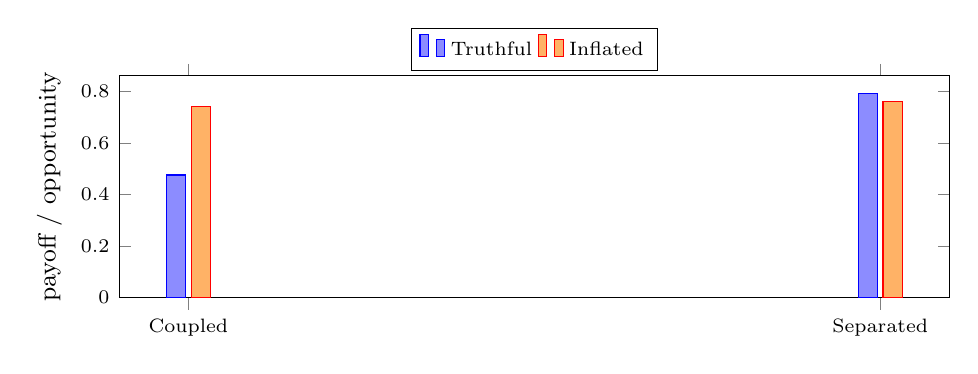
\begin{tikzpicture}
\begin{axis}[
  ybar, width=\columnwidth, height=4.4cm,
  ymin=0, ymax=0.86,
  ylabel={payoff / opportunity},
  symbolic x coords={Coupled,Separated}, xtick=data,
  bar width=7pt, legend style={font=\scriptsize,at={(0.5,1.02)},anchor=south,legend columns=2},
  tick label style={font=\scriptsize}, label style={font=\small}
]
\addplot+[fill=blue!45] coordinates {(Coupled,0.4757) (Separated,0.7911)};
\addplot+[fill=orange!60] coordinates {(Coupled,0.7413) (Separated,0.7610)};
\legend{Truthful,Inflated}
\end{axis}
\end{tikzpicture}
\caption{Strategic simulation (500 seeds, 5,000 opportunities each). Inflation
is profitable when reports control selection, but proper-score loss dominates
when audit exposure is independent of the report.}
\Description{Grouped bar chart: in the coupled condition inflated payoff is much
higher than truthful payoff; in the separated condition truthful payoff is
slightly higher than inflated payoff.}
\label{fig:strategic}
\end{figure}

\begin{figure}[t]
\centering
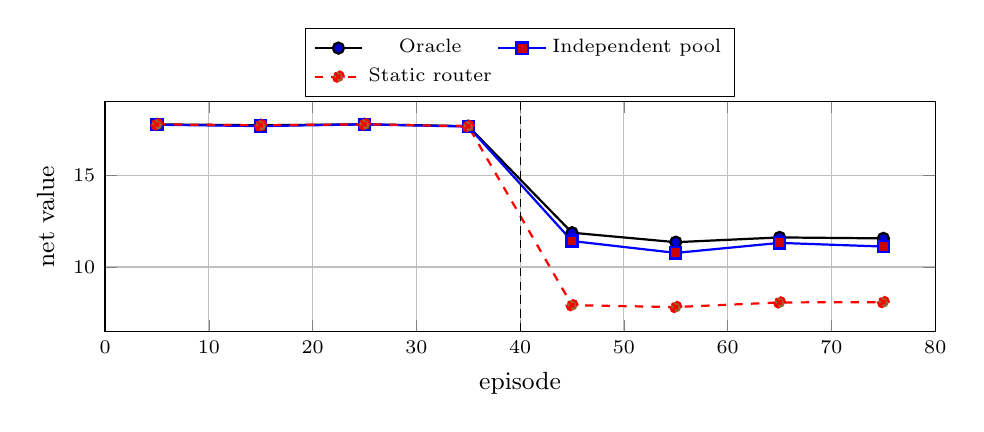
\begin{tikzpicture}
\begin{axis}[
  width=\columnwidth,height=4.5cm,
  xlabel={episode},ylabel={net value},
  xmin=0,xmax=80,ymin=6.5,ymax=19,
  legend style={font=\scriptsize,at={(0.5,1.02)},anchor=south,legend columns=2},
  tick label style={font=\scriptsize},label style={font=\small},
  grid=major
]
\addplot+[black,thick] coordinates {(5,17.759)(15,17.711)(25,17.764)(35,17.663)(45,11.866)(55,11.351)(65,11.610)(75,11.558)};
\addplot+[blue,thick] coordinates {(5,17.740)(15,17.666)(25,17.759)(35,17.641)(45,11.414)(55,10.768)(65,11.313)(75,11.113)};
\addplot+[red,dashed,thick] coordinates {(5,17.759)(15,17.711)(25,17.764)(35,17.663)(45,7.922)(55,7.823)(65,8.074)(75,8.091)};
\draw[densely dashed] (axis cs:40,6.5)--(axis cs:40,19);
\legend{Oracle,Independent pool,Static router}
\end{axis}
\end{tikzpicture}
\caption{Predeclared capability shift at episode 40. The static router does not
adapt; independent current forecasts retain most oracle value. Curves are means
over seeds in ten-episode blocks.}
\Description{Line chart with three policies. All are close before episode 40;
the static router drops sharply after the shift while the independent pool stays
near the oracle.}
\label{fig:shift}
\end{figure}

In the separate strategic experiment (Fig.~\ref{fig:strategic}), proper scoring
alone does not protect the coupled mechanism. Inflation raises selection from
0.431 to 0.708 and payoff from 0.476 to 0.741. Under report-independent audit
exposure, truth-telling yields 0.791 versus 0.761 for inflation, matching
Proposition~\ref{prop:truth}.

\section{Real-Model Confirmatory Study}

The simulator validates code paths and identifies failure modes; it cannot
establish LLM-agent effectiveness. The confirmatory study will freeze four task
families: executable code, multi-hop/tool QA, SQL/JSON transformation, and a
long-horizon agent benchmark. It will use 4--6 version-pinned workers spanning a
wide price range and at least three independent forecasters. Exact model IDs,
pricing timestamp, prompts, evaluator versions, and traces will be reported.

All policies share workers, harness, tool limits, graphs, and budgets. Required
baselines are cheapest-first, premium monolith, static cost-aware routing, Agora,
AgentLance, coupled self-report, independent equal pooling, and an oracle ceiling.
External systems will be named only when faithfully reproduced; approximations
will be labeled ``style'' or ``proxy.'' Confirmatory factors are separation,
audit rate, audit-only versus selected-only updates, and DAG versus myopic
selection. Audit budget will be randomized over
$\{0,0.5,1,2,5,10\}\%$ of execution budget.

The primary endpoint is episode settled net value including audit cost. Secondary
endpoints are pseudo-regret, Brier and log scores, calibration slope/intercept,
project completion, worst-decile value, latency, and deviation gain. A paired
pilot estimates the variance of episode-level differences; the final sample size
targets 90\% power for a smallest worthwhile effect of 5\% of oracle value. H1
uses a paired hierarchical bootstrap stratified by family; three secondary
hypotheses use Holm correction. Repeated decodes of the same task are not treated
as independent task samples. The complete preregistration is in the supplement.

\section{Limitations and Ethics}

Proposition~\ref{prop:truth} requires forecasters without side interests. A
worker-owned forecaster may manipulate allocation even if audit-scored. Audits
also consume money, energy, and possibly proprietary task data; random shadow
execution may be unacceptable in sensitive domains. Inverse propensities can
have high variance, and clipping trades variance for bias. Machine verifiers can
be gamed, project values are contestable, and benchmark success may not transfer
to live organizations. Public API prices are not private costs, so the empirical
paper must not overstate procurement incentives. Finally, our evidence is
synthetic: the real-model study can falsify the practical thesis.


\section{Conclusion}

The useful part of calibration-settled orchestration is not another LLM auction.
It is the separation of work allocation from forecast exposure when outcomes are
selectively observed. \calms{} makes that separation explicit, supplies an audit
channel and proper settlement, and exposes the audit-value frontier. Controlled
pre-experiments support the strategic diagnosis and adaptation benefit but reject
the assumption that more auditing automatically improves net value. Whether the
mechanism is practically worthwhile is now a precise, preregistered empirical
question rather than an acceptance claim.

\bibliographystyle{ACM-Reference-Format}
\bibliography{references}

\end{document}
